% Options for packages loaded elsewhere
% Options for packages loaded elsewhere
\PassOptionsToPackage{unicode}{hyperref}
\PassOptionsToPackage{hyphens}{url}
\PassOptionsToPackage{dvipsnames,svgnames,x11names}{xcolor}
%
\documentclass[
  letterpaper,
  DIV=11,
  numbers=noendperiod]{scrartcl}
\usepackage{xcolor}
\usepackage[margin=0.75in]{geometry}
\usepackage{amsmath,amssymb}
\setcounter{secnumdepth}{-\maxdimen} % remove section numbering
\usepackage{iftex}
\ifPDFTeX
  \usepackage[T1]{fontenc}
  \usepackage[utf8]{inputenc}
  \usepackage{textcomp} % provide euro and other symbols
\else % if luatex or xetex
  \usepackage{unicode-math} % this also loads fontspec
  \defaultfontfeatures{Scale=MatchLowercase}
  \defaultfontfeatures[\rmfamily]{Ligatures=TeX,Scale=1}
\fi
\usepackage{lmodern}
\ifPDFTeX\else
  % xetex/luatex font selection
\fi
% Use upquote if available, for straight quotes in verbatim environments
\IfFileExists{upquote.sty}{\usepackage{upquote}}{}
\IfFileExists{microtype.sty}{% use microtype if available
  \usepackage[]{microtype}
  \UseMicrotypeSet[protrusion]{basicmath} % disable protrusion for tt fonts
}{}
\makeatletter
\@ifundefined{KOMAClassName}{% if non-KOMA class
  \IfFileExists{parskip.sty}{%
    \usepackage{parskip}
  }{% else
    \setlength{\parindent}{0pt}
    \setlength{\parskip}{6pt plus 2pt minus 1pt}}
}{% if KOMA class
  \KOMAoptions{parskip=half}}
\makeatother
% Make \paragraph and \subparagraph free-standing
\makeatletter
\ifx\paragraph\undefined\else
  \let\oldparagraph\paragraph
  \renewcommand{\paragraph}{
    \@ifstar
      \xxxParagraphStar
      \xxxParagraphNoStar
  }
  \newcommand{\xxxParagraphStar}[1]{\oldparagraph*{#1}\mbox{}}
  \newcommand{\xxxParagraphNoStar}[1]{\oldparagraph{#1}\mbox{}}
\fi
\ifx\subparagraph\undefined\else
  \let\oldsubparagraph\subparagraph
  \renewcommand{\subparagraph}{
    \@ifstar
      \xxxSubParagraphStar
      \xxxSubParagraphNoStar
  }
  \newcommand{\xxxSubParagraphStar}[1]{\oldsubparagraph*{#1}\mbox{}}
  \newcommand{\xxxSubParagraphNoStar}[1]{\oldsubparagraph{#1}\mbox{}}
\fi
\makeatother


\usepackage{longtable,booktabs,array}
\usepackage{calc} % for calculating minipage widths
% Correct order of tables after \paragraph or \subparagraph
\usepackage{etoolbox}
\makeatletter
\patchcmd\longtable{\par}{\if@noskipsec\mbox{}\fi\par}{}{}
\makeatother
% Allow footnotes in longtable head/foot
\IfFileExists{footnotehyper.sty}{\usepackage{footnotehyper}}{\usepackage{footnote}}
\makesavenoteenv{longtable}
\usepackage{graphicx}
\makeatletter
\newsavebox\pandoc@box
\newcommand*\pandocbounded[1]{% scales image to fit in text height/width
  \sbox\pandoc@box{#1}%
  \Gscale@div\@tempa{\textheight}{\dimexpr\ht\pandoc@box+\dp\pandoc@box\relax}%
  \Gscale@div\@tempb{\linewidth}{\wd\pandoc@box}%
  \ifdim\@tempb\p@<\@tempa\p@\let\@tempa\@tempb\fi% select the smaller of both
  \ifdim\@tempa\p@<\p@\scalebox{\@tempa}{\usebox\pandoc@box}%
  \else\usebox{\pandoc@box}%
  \fi%
}
% Set default figure placement to htbp
\def\fps@figure{htbp}
\makeatother





\setlength{\emergencystretch}{3em} % prevent overfull lines

\providecommand{\tightlist}{%
  \setlength{\itemsep}{0pt}\setlength{\parskip}{0pt}}



 


\KOMAoption{captions}{tableheading}
\usepackage{../latex_packages/abbreviations}
\usepackage{fancyhdr}
\pagestyle{fancy}
\let\headrule\empty
\let\footrule\empty
\lhead{{\bfseries CSC\,413}}
\chead{{\bfseries Exercises - Week 2}}
\rhead{{\bfseries Shkurti / Gilitschenski}}
\lfoot{{}}
\cfoot{{\thepage}}
\rfoot{{}}
\makeatletter
\@ifpackageloaded{caption}{}{\usepackage{caption}}
\AtBeginDocument{%
\ifdefined\contentsname
  \renewcommand*\contentsname{Table of contents}
\else
  \newcommand\contentsname{Table of contents}
\fi
\ifdefined\listfigurename
  \renewcommand*\listfigurename{List of Figures}
\else
  \newcommand\listfigurename{List of Figures}
\fi
\ifdefined\listtablename
  \renewcommand*\listtablename{List of Tables}
\else
  \newcommand\listtablename{List of Tables}
\fi
\ifdefined\figurename
  \renewcommand*\figurename{Figure}
\else
  \newcommand\figurename{Figure}
\fi
\ifdefined\tablename
  \renewcommand*\tablename{Table}
\else
  \newcommand\tablename{Table}
\fi
}
\@ifpackageloaded{float}{}{\usepackage{float}}
\floatstyle{ruled}
\@ifundefined{c@chapter}{\newfloat{codelisting}{h}{lop}}{\newfloat{codelisting}{h}{lop}[chapter]}
\floatname{codelisting}{Listing}
\newcommand*\listoflistings{\listof{codelisting}{List of Listings}}
\makeatother
\makeatletter
\makeatother
\makeatletter
\@ifpackageloaded{caption}{}{\usepackage{caption}}
\@ifpackageloaded{subcaption}{}{\usepackage{subcaption}}
\makeatother
\usepackage{bookmark}
\IfFileExists{xurl.sty}{\usepackage{xurl}}{} % add URL line breaks if available
\urlstyle{same}
\hypersetup{
  colorlinks=true,
  linkcolor={blue},
  filecolor={Maroon},
  citecolor={Blue},
  urlcolor={Blue},
  pdfcreator={LaTeX via pandoc}}


\author{}
\date{}
\begin{document}


\subsection{Exercise 1 - Eigenvectors and
Eigenvalues}\label{exercise-1---eigenvectors-and-eigenvalues}

For a square matrix \(\fA\) of size \(n \times n\), a vector
\(\fu_i \neq 0\) which satisfies \begin{equation}
\fA\fu_i = \la_i \fu_i
\label{eq:eigen}
\end{equation} is called a \emph{eigenvector} of \(\fA\), and \(\la_i\)
is the corresponding \emph{eigenvalue}. For a matrix of size
\(n \times n\), there are \(n\) eigenvalues \(\la_i\) (which are not
necessarily distinct).

Show that if \(\fu_1\) and \(\fu_2\) are eigenvectors with equal
corresponding eigenvalues \(\la_1 = \la_2\), then
\(\fu = \al \fu_1 + \be \fu_2\) is also an eigenvector with the same
eigenvalue.

\subsubsection{Solution}\label{solution}

Because \(\la_1=\la_2\), we will write \(\la\) for simplicity. The
result is obtained by applying the definition of eigenvalues and
distributivity via \begin{equation*}
\fA\fu 
  = \fA (\al \fu_1 + \be \fu_2) 
  =   \al \fA \fu_1 + \be \fA \fu_2
  =   \al \la \fu_1 + \be \la \fu_2
  =   \la (\al\fu_1 + \be \fu_2)
  =   \la \fu .
\end{equation*}

\subsection{Exercise 2 - Variance and
Expectation}\label{exercise-2---variance-and-expectation}

\begin{enumerate}
\def\labelenumi{(\alph{enumi})}
\item
  Given a set of vectors \(\{\fx_i\}_{i=1}^N\). Show that their
  empirical mean is equivalent to
  \[\hmu=\argmin_\fmu \sum_i \|\fx_i - \fmu\|^2.\]
\item
  There are two equivalent definitons of variance of a random variable.
  The first one is \(\Var(X) := \E[(X - \E[X])^2]\) and the second is
  \(\Var(X) = \E[X^2] - \E[X]^2\). Show that these two definitions
  actually are equivalent.
\end{enumerate}

\subsubsection{Solution}\label{solution-1}

\begin{enumerate}
\def\labelenumi{(\alph{enumi})}
\item
  The key idea here is to compute the gradient of the objective function
  and solve for \(\fmu\). The gradient is obtained by applying the chain
  rule resulting in
  \[0=\nabla_\fmu \sum_i \|\fx_i - \fmu\|^2 = -2 \sum_i (\fx_i - \fmu) .\]
  Now, we solve this for \(\fmu\) to obtain
  \[\fmu = \frac{1}{N} \sum_i \fx_i .\]
\item
  Here, we simply need to apply some algebraic manipulations to show
  that the two definitions are equivalent. We start with the first
  definition and expand the square: \begin{align*}
  \E[(X - \E[X])^2] 
    &= \E\li[X^2 - 2X\E[X]+\E[X]^2\ri] \\
    &= \E\li[X^2\ri] - \E[2X\E[X]]+\E\li[\E[X]^2\ri]\\
    &= \E\li[X^2\ri] - 2\E[X]\E[X]+\E[X]^2\\
    &= \E\li[X^2\ri] - \E[X]^2
  \end{align*}
\end{enumerate}

\subsection{Exercise 3 - Linear
Regression}\label{exercise-3---linear-regression}

\begin{enumerate}
\def\labelenumi{(\alph{enumi})}
\item
  In the linear regression model with one feature, we have the following
  model/hypothesis: \[y = f(x) = w x + b\] \hspace{0pt}with parameters,
  \(w\) and \(b\), which we wish to find by minimizing the cost:
  \[\mathcal{E}(w, b) = \frac{1}{2N}\sum_i ((w x^{(i)} + b) - t^{(i)})^2\]
  What are the derivatives \(\frac{\partial \mathcal{E}}{\partial w}\)
  and \(\frac{\partial \mathcal{E}}{\partial b}\)?
\item
  In the linear regression model with many features, we have the
  following model/hypothesis: \[y = f(x) = {\bfseries w}^\top {\bfseries x}+ b\]
  with parameters, \({\bfseries w} = [w_1, w_2, \dots w_d]^T\) and \(b\),
  which we wish to find by minimizing the cost:
  \[\mathcal{E}({\bfseries w}, b) = \frac{1}{2N}\sum_i ((\fw^\top \fx^{(i)}+b) - t^{(i)})^2\]
  What is the derivative \(\frac{\partial \mathcal{E}}{\partial w_j}\)
  for a weight \(w_j\)?
\end{enumerate}

\subsubsection{Solution}\label{solution-2}

\begin{enumerate}
\def\labelenumi{(\alph{enumi})}
\item
  We obtain the derivative with respect to \(w\) directly using the
  chain rule resulting in \[
  \frac{\partial \mathcal{E}}{\partial w} 
    = \frac{1}{N}\sum_i x^{(i)}((w x^{(i)} + b) - t^{(i)}) 
  \] Similarly, the derivative with respect to \(b\) is \[
  \frac{\partial \mathcal{E}}{\partial b} 
    = \frac{1}{N}\sum_i ((w x^{(i)} + b) - t^{(i)})
  \]
\item
  The derivative with respect to \(w_j\) is \[
  \frac{\partial \mathcal{E}}{\partial w_j} 
    = \frac{1}{N}\sum_i x_j^{(i)}((\fw^\top \fx^{(i)}+b) - t^{(i)})
  \]
\end{enumerate}

\subsection{Exercise 4 - Gradients and Computation
Graphs}\label{exercise-4---gradients-and-computation-graphs}

\begin{enumerate}
\def\labelenumi{(\alph{enumi})}
\item
  Compute the \(\frac{\partial \mathcal{L}}{\partial w_j}\) gradient of
  \(\mathcal{L}\) with respect to a \(w_j\) in the following
  computation: \begin{align*} 
    \mathcal{L}(y, t) &= - t \log(y) - (1-t) \log(1-y) ,
  & y &= \sigma(z) ,
  &  z &= {\bf w}^\top {\bf x} .
    \end{align*}
\item
  Draw the computation graph for the following neural network, showing
  the relevant scalar quantities. Assume that
  \(\fy, \fh, \fx \in \mathbb{R}^2\) \begin{align*}
    \mathcal{L} &= \frac{1}{2}\sum_k (y_k - t_k)^2 , 
  & y_k &= \sum_i w_{ki}^{(2)} h_i + b_k^{(2)} , 
  & h_i &= \sigma(z_i) ,
  & z_i &= \sum_j w_{ij}^{(1)} x_j + b_i^{(1)} .
    \end{align*}
\end{enumerate}

\subsubsection{Solution}\label{solution-3}

\begin{enumerate}
\def\labelenumi{(\alph{enumi})}
\item
  Applying the chain rule, we have

  \[ \frac{\partial \mathcal{L}}{\partial w_j} = \frac{\partial \mathcal{L}}{\partial y} \frac{\partial y}{\partial z} \frac{\partial z}{\partial w_j} \]

  Looking at each term individually yields \[
  \begin{aligned}
  \frac{\partial \mathcal{L}}{\partial y} 
    &= \frac{\partial}{\partial y} [-t \log(y) - (1 - t) \log(1 - y)] 
    = - \frac{t}{y} + \frac{1 - t}{1 - y}\\
  \frac{\partial y}{\partial z} 
    &= \frac{\partial \sigma(z)}{\partial z} 
    = \sigma(z) (1 - \sigma(z))
    = y (1 - y)\\
  \frac{\partial z}{\partial w_j} 
    &= \frac{\partial}{\partial w_j} (w^\top x) = x_j
  \end{aligned}
  \]

  Bringing it all together yields: \[
  \begin{aligned}
  \frac{\partial \mathcal{L}}{\partial w_j} 
    &= \left( - \frac{t}{y} + \frac{1 - t}{1 - y} \right) \cdot y (1 - y) \cdot x_j \\
    &= (-t + ty + 1 - t - y + ty) x_j \\
    &= (y - t) x_j
  \end{aligned}
  \]
\item
  The computation graph is given in the figure below.
\end{enumerate}

\begin{figure}[H]

{\centering 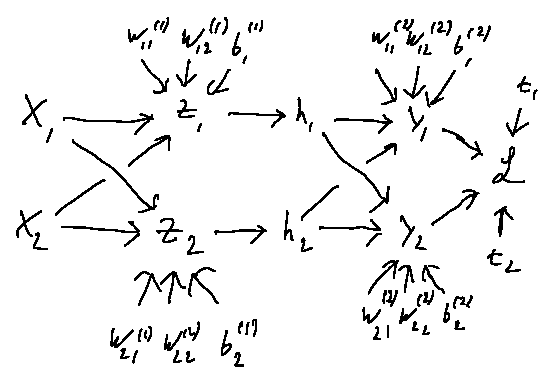
\includegraphics[width=0.5\linewidth,height=\textheight,keepaspectratio]{nn-compgraph-drawing.eps}

}

\caption{Computation graph for exercise 4 (b)}

\end{figure}%




\end{document}
